\section{Technical Implementation}

% Do these need references?
Discovery Service is implemented with Python programming language and Flask Web framework. They were chosen because all of the components in Cloudify are also written in Python and Flask is used primarily for providing REST APIs. Even though Discovery Service does not provide any REST APIs, Flask is used for configuration management and source code organisation. Naturally, if need arises in the future to expand Discovery Service with a REST API, the development work is streamlined because of the framework.

In addition to Python program, Discovery Service relies on Redis \cite{Redis} as an in-memory key-value storage. Redis is a completely separate process in addition to Discovery Service. The preferred way of deploying Redis is in a docker container as it doesn't require installation or configuration save for exposing a correct port in the container and specifying Redis' address to Discovery Service. Redis could also be installed in the host system or even a remote system, though latter option has no practical purpose due to network latency as Redis achieves its high performance by storing values in the memory instead of disk.

\begin{figure}[ht!]
\centering
  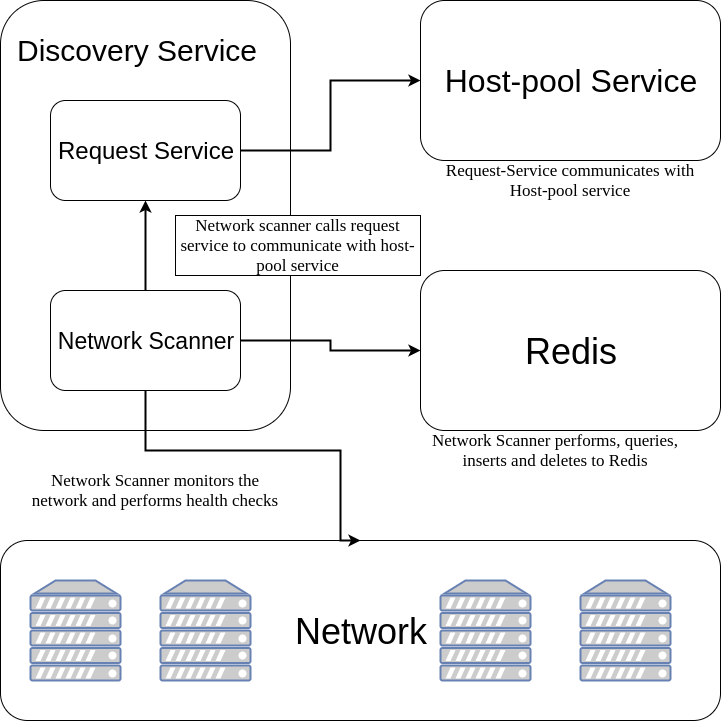
\includegraphics[width=12cm,height=12cm, keepaspectratio]{Discovery-service-communication.png}
  \caption{The communication relationships between Discovery Service and other components}
  \label{fig:communications}
\end{figure}

On the source code level, Discovery Service consists of two major components: The network scanner and request service. The network scanner is given a subnet as a parameter and it constantly sniffs the network detecting joining and already present devices and keeping track of them. Its other task is to periodically send health checks to known devices and if a health check fails enough times, it removes the given device from the logical host pool. Request service is responsible for sending HTTP requests to the Cloudify Host-pool service. It is called by the request service and it runs asynchronously. In addition to HTTP requests, it performs checks to ensure that the state of Discovery service's and Host-pool service's databases correlate.

The communication relationships between different components in the system are depicted in figure \ref{fig:communications}. The source code for Discovery Service as well as the documentation can be found at \url{https://bitbucket.org/Fleuri/discoveryserviceforcloudify/src/master/}

\subsection{Network Scanner}

The Network Scanner has two main functions, sniffer and pinger, and they run concurrently on two threads. Sniffer listens to ARP packets in the network and upon receiving one, stores the details of the sender device. Pinger function periodically sends ARP pings to previously discovered device and keeps track of their successes, eventually removing unresponsive devices from the logical host pool. In addition to two main functions there's a start-up function that initialises both local Redis storage and the Host-pool service's database. It pings all of the IP addresses in the given IP range and stores the found device details to databases.

\subsubsection{Sniffer}

Sniffer is started in its own thread during the start up sequence of the Discovery Service. It uses \textit{Scapy} library \cite{scapy} for Python. Sniffer function is given three arguments: 

\begin{enumerate}
\item \textbf{The network interface} which the Sniffer listens to for incoming packets.
\item \textbf{The callback function} which details further instructions to perform when a packet is caught.
\item \textbf{The filter} which restricts the type of packets caught.
\end{enumerate}

Only the interface can be set by the user of the Discovery Service. The callback function is the core application logic of the sniffer and the Discovery Service itself relies on sniffing ARP packets and therefore the filter is set accordingly.

When it comes to programming logic, the callback function is the most interesting part of the sniffer. Its purpose is to evaluate whether an ARP request comes from a new or know device and store details about them. When the function receives an ARP packet it first filters out packets that are not standard ARP requests. There are two such cases: ARP Probe \cite{rfc5227}, in which the source IP address or hardware address of the ARP request is \textit{0.0.0.0} or \textit{00:00:00:00:00:00} respectively, and gratuitous ARP in which the hardware address is \textit{ff:ff:ff:ff:ff:ff}. The user can also define a list of IP and hardware addresses which the Discovery Service should ignore i.e. devices on which Cloudify should not run workloads. Such devices include the host on which Cloudify manager runs and network devices such as routers.

Next the function checks whether the packet's origin is an already known host by querying Redis. If the host is not previously known or if it is a known device with a changed IP address, the function starts a new thread to add or patch the host to the Host-pool service. See section \ref{requestservice}.

Whether the packet's origin host is known or not, the next step in the function is to insert values extracted from the packet to Redis. The data structure Discovery service uses is simple, being a hash table with the devices' hardware address being a key and value being a dictionary object consisting of the given device's IP address and the number of failed ping attempts. See section \ref{pinger} for more details. If the packet's origin is a new host, its key and values are inserted to the data store with number of failed pings always being zero. If a device is already known, its hardware address is already stored to Redis and therefore its values are modified: in most cases only the failed ping count is reset to zero but there could be cases in which the device's IP address has changed and it is updated here accordingly. Algorithm \ref{fig:snifferalgo} details the structure of the function. Note that both adding a new host and patching an already known host is done in the same Request Service function. See section ~\ref{addtohostpool} for details.

\begin{algorithm}[H]
\label{fig:snifferalgo}
\begin{center}
\end{center}
\KwIn{Packet}
\If{Packet is an ARP packet}{
	\If{Packet is not an ARP Probe or Gratuitous ARP}{
	 	\If{Hardware address not found in Redis or IP address not found in Redis}{
	 	RequestService.Register\_a\_new\_host()\;
	 	}
		Redis.store(Packet.HardwareAddress: \{ip\_address: Packet.IPAddress, ping\_timeouts: 0\})\;
	}
}
\caption{Sniffer Callback Function}
\end{algorithm}

\subsubsection{Pinger} \label{pinger}

Pinger function is started in its own thread in the Network Scanner. Its responsibility is to keep track of the health of the nodes in the network. If Pinger discovers an unreachable node, it is removed from both Redis' and Host-pool service's storage.

Pinger periodically works through a list of known hosts in the network sending an ARP ping to each host. Upon receiving a response it resets the corresponding host's ping time-out counter to zero. If Pinger does not receive a response, it increments the given hosts' ping time-out by one. If after this operation the time-out crosses the given ping time-out threshold, the host is assumed to have disconnected from the network and is removed from the storage. After Pinger has pinged every host in the network, the process waits for a given ping interval after which it restarts the process.

The user gives inputs two parameters in a configuration file for Pinger to use: \textit{ping\_timeout\_threshold} and \textit{ping\_interval}. Ping\_timeout\_threshold specifies the maximum consecutive ping failures that can occur before a host is marked unreachable and removed from storage. Ping\_interval is the duration in seconds of which Pinger waits after each round of pinging the network. The more detailed presentation of the function is presented in the algorithm ~\ref{fig:pingeralgo}.

\begin{algorithm}[H]
\label{fig:pingeralgo}
\begin{center}
\end{center}

\While{True}{
	\ForEach{host in Redis}{
		timeouts = host.ping\_timeouts\;
		response = Ping(host)\;
	 	\If{response}{
	 		Redis.patch(host, \{ping\_timeouts: 0\})\;
	 	}
	 	\Else{
	 		timeouts++\;
	 		\If{timeouts >= ping\_timeout\_threshold}{
	 			RequestService.delete(host)\;
	 			Redis.delete(host)\;
		} \Else {
			Redis.patch(host, \{ping\_timeouts: timeouts\}\;		
		}		
	}
}
Sleep(ping\_interval)\;
}

\caption{Pinger Algorithm}

\end{algorithm}

\subsection{Request Service} \label{requestservice}

Request Service is responsible of communication between the Discovery Service and Host-pool Service. As seen on figure ~\ref{fig:communications}, it is called by Network Scanner and it makes requests to Host-pool Service. The REST API Host-pool Service provides is quite succinct but provides a typical CRUD interface for handling nodes in the network. The methods are as follows\footnote{\textit{Note: Paths are relative to Host-pool service base URL e.g. localhost:8081/hosts}} 

\begin{description}

\item[\textbf{[GET] /hosts}] \hfill \\
GET request to /hosts returns a JSON list of hosts and their details. Also accepts certain filters.

\item[\textbf{[POST] /hosts}] \hfill \\
POST request to /hosts with a valid JSON array will add one or more hosts to Host-Pool service's storage See listing ~\ref{lst:JSONformat} for the JSON schema definition. Returns Id’s of the new host or hosts.

\item[\textbf{[GET] /host/{id}}] \hfill \\
Returns details of a single host corresponding to the ID number.

\item[\textbf{[PATCH] /host/{id}}] \hfill \\
PATH request allows updating specified fields of a host with the given ID.

\item[\textbf{[DELETE] /host/{id}}] \hfill \\
Removes the host with given ID from Host-pool service's storage.

\item[\textbf{[POST] /host/allocate}] \hfill \\
This API call allocates a host to be used by the Cloudify Manager.

\item[\textbf{[DELETE] /host/{id}/deallocate}] \hfill \\
This returns a previously allocated host back to the host pool to be reallocated again.

\end{description}

Request Service interacts with all of the REST API endpoints except for allocation and deallocation endpoints which are interacted by Cloudify Manager's Host-pool plugin.

On source code level a typical Request Service function either makes an HTTP request to a certain endpoint, possibly with an ID corresponding to a host in the network, or constructs a JSON payload and sends that along with a POST request. Programmatic challenge in Request Service rises from the fact that the data model Host-pool service accepts is significantly more robust than that of the Discovery service, as can be seen on listing ~\ref{lst:JSONformat}. If Discovery Service's data model as seen on listing ~\ref{lst:discoformat} was a subset of Host-pool service's, handling data in Request Service would be trivial. However as Discovery Service's data model uses hardware addresses as unique identifiers whereas Host-Pool Service attaches a running number to each host. Hardware addresses are used as they are immutable in the cluster use-case and Discovery Service accounts for possibly changing IP addresses. However, Hardware addresses are by to Host-pool Service implicitly, as Discovery Service assigns each host's hardware address as a value for 'name' key. 

\begin{lstlisting}[language=json,firstnumber=1, caption={JSON schema accepted by the Host-pool Service for a single host}, captionpos=b, label=lst:JSONformat]
hosts: {
	id: Integer
	name: String
	os: String
	endpoint {
		ip : String
		protocol: String
		port: Integer	
	}
	credentials: {
		username: String
		password: String
		key: String
	}
	tags: Array
	allocated: Boolean
	alive: Boolean
}

NOTES:
- name is an arbitrary string, but Discovery Service assigns the host's hardware address as the value of name.
- os can be either 'linux' or 'windows'. Other values are invalid.
- endpoint.ip has to be a valid IP address range with CIDR notation. If a range is defined, Host-pool Service considers each unique IP address a single host.
- protocol can be either 'winrm-http', "'winrm-https' or 'ssh', but Host-pool service does not explicitly force this.
- Host-pool Service manages id, allocated and alive fields. For User, all other fields except credentials.password, credentials.key and tags are obligatory.
- In addition to 'hosts' key, Host-pool Service also accepts 'defaults' key. 'defaults' can contain the same keys as 'hosts'. If 'defaults' is provided, its values are appended to each host which has respective undefined values. id, allocated and alive cannot be provided as defaults.

\end{lstlisting}

\begin{lstlisting}[language=json,firstnumber=1, caption={Discovery Service data format for a single host}, captionpos=b, label=lst:discoformat]
hwaddress: {ip_address: "string", ping_timeouts:  "integer"}
\end{lstlisting}

\subsubsection{Id checking}

Due to differing identifiers, certain functions are implemented to keep the two data stores synchronized. A \verb|get_id()| -function retrieves a JSON object of hosts as depicted in algorithm ~\ref{fig:get_id}. Then it compares stored IP addresses for each host or until a match is found after which the ID is returned. If hardware address is passed as an argument, the function also compares it to \emph{name} -field's value, as Discovery Service names hosts in Host-pool Service after their hardware addresses. Hardware address check is used when Network Scanner finds an already known host with a changed IP address and calls Request Service to patch it to Host-pool Service. The ID itself is used for REST API calls that are directed at a single host.

\begin{algorithm}[H]
\label{fig:get_id}
\begin{center}
\end{center}
\KwIn{ip\_address}
\KwIn{hardware\_address = None}
\ForEach{host in RequestService.get\_hosts()}{
	\If{host.endpoint.ip is ip\_address or
		name is not None and 
		host.name is hardware\_address}{
	 		\Return{host.id}\;
	 	}
}
\Return{None}\;
\caption{get\_id -function compares stored IP addresses and optionally hardware addresses to find out the corresponding ID number in Host-pool Service.}
\end{algorithm}

\subsubsection{Adding a new host to Host-pool Service} \label{addtohostpool}

When Network Scanner detects a new host, it adds it to Redis key-value storage and starts a Request Service routine \verb|register_a_new_host| depicted in algorithm ~\ref{fig:addhost} in
a new thread to add the details also to Host-pool service. If a new IP address is detected but with an existing hardware address, the same routine is called. The \verb|register_a_new_host| function takes existing hosts into account and branches to patching function if need be. However, IP address changing for a host is a rare occasion and thus the function branching logic is done in Request Service for optimisation and maintaining source code readability.

\begin{algorithm}[H]
\label{fig:addhost}
\begin{center}
\end{center}
\KwIn{ip\_address}
\KwIn{hardware\_address = None}
{
stored\_id = get\_id(ip\_address, hardware\_address)
\If{stored\_id is None} {
	data = *formatted json object corresponding to host's details*\;
	response = *POST request to Host-pool Service with 'data' as payload.*\;
	\Return{response.json, message}
} \Else {
	\Return{RequestService.patch\_a\_host(stored\_id, ip\_address, hardware\_address)}
}
}

\caption{get\_id -function compares stored IP addresses and optionally hardware addresses to find out the corresponding Id number in Host-pool Service.}
\end{algorithm}

\subsubsection{Limitations and assumptions of the Discovery Service}

At its current prototypical state Discovery Service makes certain assumptions about the physical hosts in the cluster.
Namely hosts are assumed to have Linux as an operating system (Distribution can vary) and a default user name and a password, those being 'centos' and 'admin' respectively. In addition hosts are required to be running an SSH server which is a requirement enforced to Linux hosts by Cloudify itself. Discovery Service requires that the standard port 22 for SSH is open.

\subsubsection{Patching a host}

Host-pool Service allows duplicate hosts, a feature which can be regarded as an oversight by the Host-pool Service developers. Discovery Service enforces that single host has only a single recorded IP address stored in the system. Therefore, if Discovery Service detects a host which has an already existing IP or Hardware Address, but the other one differs from the already stored one, Discovery Service will patch the given address with the new one. The patching to Redis is done in the Network Scanner as previously seen in algorithm~\ref{fig:snifferalgo}. The patching to Host-pool Service is depicted in algorithm~\ref{fig:patch}

\begin{algorithm}[H]
\label{fig:patch}
\setlength{\AlCapSkip}{1em}
\begin{center}
\end{center}
\KwIn{id}
\KwIn{ip\_address}
\KwIn{hardware\_address}

data = \{\}\;
host = RequestService.get\_a\_host(id)\;

\If{host.ip != ip\_address} {
	data['ip'] = ip\_address\;
} 
\ElseIf{host.name != hardware\_address}{
	data['name'] = hardware\_address\; 
}
\Else { \Return{ \{\}, message}}

response = *PATCH request to Host-pool Service with 'data' as payload.*\;
\Return {response.json, message}

\caption{patch\_a\_host function is called by register\_a\_new\_host when Discovery Service detacts a host whose IP address has changed or a new host which uses the same IP address as another host previously.}

\end{algorithm}
\vspace*{1em}

The function \verb|patch_a_host| takes three arguments: The Id of the host in Host-pool Service, host's IP address and its hardware. Then it retrieves the host's details from Host-pool Service in JSON format and compares the IP addresses received as an argument and retrived from Host-pool Service. If they do not match, the argument IP address is patched as the new value to Host-pool Service using the REST function. 